\section{RxJS: Reactive Extensions For JavaScript}
Rx ist eine Library, die für zahlreiche Programmiersprachen zur Verfügung gestellt wird. Diese finden sowohl in der Frontend als auch in der Backend-Implementierung Anwendung. In dieser Arbeit wird der Fokus auf RxJS geworfen. Diese Library ist eine Erweiterung speziell für Javascript/Typescript. RxJS erlaubt es mit Hilfe von Observable-Sequenzen Event-basierte Programme zu erstellen. Dabei wird dieser Ansatz auch als reactive Programming definiert. Neben der Kernfunktionalität von Observables werden auch Subjects und Schedulers geboten. Sollte man von reactive Programming noch nichts gehört haben, dann wird die größte Herausforderung sein \glqq{}reactive\grqq{} zu denken.

\subsection{Reactive Programming}
Im Kern ist reactive Programming ein Programmierparadigma. Hierbei richtet sich das Entwickeln mit asynchronen Datenflüssen. Als Beispiel für eine reaktive Anwendung kann Excel genommen werden. Ändert man einen Wert in einer Zelle, ändert sich auch der Wert in der Summenzelle. Die Zelle, deren Wert geändert wurde, löst ein Event aus, den die Summen-Zelle empfängt. Daraufhin findet eine Neuberechnung statt.\cite{reactive-programming-beispiel} Laut der offiziellen Dokumentation richtet sich ReactiveX nach dem Beobachter-Muster (engl. Observer-Pattern). Das Observer-Pattern ist ein Entwurfsmuster, in der Änderungen eines Objektes (Subjects genannt) an einer Liste abhängiger Strukturen weitergereicht wird. Diese abhängige Strukturen (Observers) werden bei jeder Zustandsveränderung informiert. Eine Veränderung eines Objekts kann hierbei gleichgesetzt werden mit einem Datenfluss. Datenflüsse können aus verschiedensten Operationen entstehen wie z.B. Klick-Events, Variablen, Cache etc. Als Observer kann man sich in diesem Datenfluss einhängen und entsprechend reagieren.\cite{rx-intro} Rx bietet eine enorme Menge an Funktionen diese Datenflüsse zu bearbeiten/manipulieren (siehe Sektion Operatoren). Diese Operatoren komplett abzudecken wird in dieser Arbeit unmöglich sein, jedoch wird nach dem behandeln dieses Kapitels ein gewisses Grundverständnis für neue Operatoren entstehen und wie diese in Folge anzuwenden sind. Die grundlegenden Konzepte, um asynchrone Events in RxJS zu steuern, sind:

\begin{itemize}
    \item Observable: Repräsentiert die Idee einer abrufbaren Sammlung, in der zukünftige Werte oder Events gelagert sind.
    \item Observer: Eine Sammlung von Callbacks die, die  aus dem Observable-Stream gelieferten Werte, abrufen.
    \item Subscription: Repräsentiert das Aufrufen eines Observable.
    \item Operators: Funktionen, die das Verhalten von Observable-Streams beeinflussen.
    \item Subjects: Eventgeneratoren, die Events an zuhörende Observer zurückgibt. Im Gegensatz zu Observables, ist hier ein Multicasting der Werte an die Observer möglich.
    \item Schedulers: Steuerungsmechanismen die bestimmen, wann eine Subscription startet und wann Werte aus dem Stream an die Observer übermittelt werden.
\end{itemize}

\subsection{Observables}

Observables sind eine träge Sammlung von multiplen Werten. Sie füllen den fehlenden Platz in der unten stehenden Tabelle:

\begin{center}
    \begin{tabular}{| l | l | l |}
    \hline
    & \textbf{Einzelne-} & \textbf{Multiple Werte} \\ \hline
    \textbf{Pull/synchron} & Funktionen & Iterables (Arrays, Strings, ...) \\ \hline
    \textbf{Push/asynchron} & Promises & Observables  \\ \hline
    \end{tabular}
\end{center}

\noindent
Das Push- und Pull-Prinzip beschreibt dabei wie ein Daten-Produzent mit dem Daten-Verarbeiter kommuniziert. In \textbf{Pull-Systemen} bestimmt der Verarbeiter, wann die Daten vom Ersteller angenommen werden. Der Ersteller selbst weiß nicht wann die Daten angefragt werden.
Jede Javascript Funktion unterliegt einem Pull-System. Die Funktion ist ein Verarbeiter von Daten, und der Code der die Funktion aufruft, verarbeitet diese.\\

\noindent
Das \textbf{Push-Prinzip} wird im nächsten Beispiel deutlich. Vor dem Ausführen des Beispiels muss folgend konfiguriert werden:

\begin{center}
     async-patterns$\,\to\,$ webpack.config.js
\end{center}

\begin{figure}[H]
\begin{lstlisting}[basicstyle=\small]
module.exports = {
    mode: 'development',
    entry: './src/modules/rxjs/observable-introduction.ts',
    ...
}
\end{lstlisting}
\end{figure}

\begin{figure}[H]
\begin{lstlisting}[basicstyle=\small]
const root: Observable<number> = RxJS.Observable.create((observer) => {
    observer.next(1);
    observer.next(2);
    observer.next(3);
    setTimeout(() => {
        observer.next(4);
        observer.complete();
    }, 1000);
});

console.log('Before subscribe');
root.subscribe({
    next: x => console.log('Value: ' + x),
    error: err => console.error('Error occurred: ' + err),
    complete: () => console.log('Done!'),
});
console.log('After subscribe');
\end{lstlisting}
\caption{Observable können sich sowohl synchron als auch asynchron verhalten.}
\end{figure}

\noindent
Das Observable-Objekt repräsentiert eine Kollektion die Werte zu seinen Beobachtern offenbart. In diesem Beispiel wird ein Observable erstellt, dass sofort (synchron) die Werte 1, 2 und 3 produziert, sobald die Subscription gestartet wird. Der vierte Wert wird asynchron übermittelt und das Observable daraufhin geschlossen. Wichtig ist, dass man sich ein Observable-Stream nur mit der subscribe()-Methode anschließen kann. Die Konsole gibt die Werte in folgender Reihenfolge aus:

\begin{figure}[H]
\begin{center}
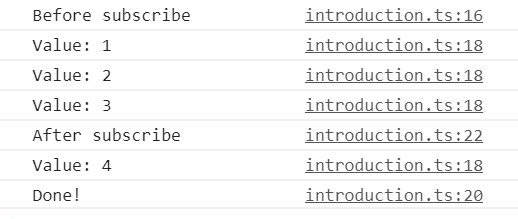
\includegraphics{observable-create-console}
\end{center}
\end{figure}

\noindent
Bei einer Subscription können drei verschiedene Events auftreten und somit drei verschiedene Funktionen aufrufen:

\begin{itemize}
\item next: () =\textgreater Wenn ein Wert ausgegeben wird,
\item error: () =\textgreater Wenn ein Fehler ausgegeben wird,
\item complete: () =\textgreater Wenn sich der Stream schließt.
\end{itemize}

\noindent
In Push-Systemen steuert der Daten-Produzent, wann die Daten an die Zuhörenden übermittelt werden. Der Daten-Verarbeiter weiß dabei nicht, wann die Daten ankommen. Promises sind ein typisches Beispiel für Push-Systeme. Ein Promise (Produzent) übermittelt einen eingetroffenen Wert an angeschlossene Callbacks( Verarbeiter). Ungleich wie mit Funktionen bestimmen Promises, wann die Werte an die Callbacks weitergereicht wird. Observables zählen zu einem neuen Push-System in Javascript. Im Gegensatz zu Promises emittieren Observables multiple Werte in Form von Streams. Zur Unterscheidung:

\begin{itemize}
\item Eine Funktion ist eine träge ausführende Operation, die beim Abruf ein Wert synchron zurückgibt.
\item Ein Promise ist eine Operation die einen eventuell eintreffenden oder nicht-eintreffenden Wert zurückgibt.
\item Ein Observable ist eine träge ausführende Operation, dass synchron oder asynchron keine oder potenziell unendlich viele Werte ab dem Zeitpunkt des Aufrufs zurückgibt.
\end{itemize}

\noindent
Hierbei stellt sich die Frage, was bedeutet träge? Träge Funktionen, im englischen auch als \textit{lazy Functions} bezeichnet, sind Funktionen die erst bei ihrem Aufruf Werte produzieren. Beispiel:

\begin{figure}[H]
\begin{lstlisting}[basicstyle=\small]
function foo() {
    console.log('Hello');
    return 42;
}

const x = foo.call(this); // same as foo()
console.log(x);
const y = foo.call(this); // same as foo()
console.log(y);
\end{lstlisting}
\caption{Funktionen sind träge. \cite{lazy-functions}}
\end{figure}

\begin{figure}[H]
\begin{lstlisting}[basicstyle=\small]
const foo = Rx.Observable.create((observer) => {
  console.log('Hello');
  observer.next(42);
});

foo.subscribe((x) => {
  console.log(x);
});
foo.subscribe((y) => {
  console.log(y);
});
\end{lstlisting}
\caption{Observables verhalten sich gleich.}
\end{figure}

\noindent
Der Output bleibt immer derselbe:
\begin{figure}[H]
\begin{center}
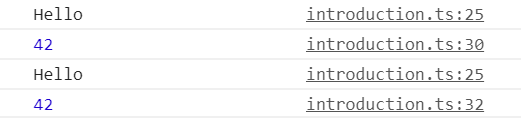
\includegraphics{observable-lazy-console}
\end{center}
\end{figure}

\noindent
Das liegt daran, da sowohl Funktionen als auch Observables träge sind. Die Operationen innerhalb beider Typen findet erst beim Aufruf statt. Mit anderen Worten: Das starten einer Subscription ist analog zum Aufruf einer Funktion. Entgegen der Annahme, dass Observables ausschließlich asynchron operieren können diese ebenfalls synchron Werte ausgeben (siehe Abb. 25).

\subsubsection{Hot- vs. Cold-Observables}

\subsection{Operatoren}
Wenn es um Operatoren geht, sind diese die wahre Stärke der Observables. Operatoren gibt es in verschiedenen Kategorien: Sie manipulieren das Stream-Verhalten oder bearbeiten die Werte innerhalb eines Streams. Eines haben Operatoren gemeinsam. Wenn ein Operator an einem Stream angewendet wird, wird ein neuer Stream erstellt. Das liegt daran, dass Streams an sich unveränderbar (engl. immutable) sind. ....

\subsection{Subjects}
\subsubsection{Unicast vs. Multicast}









